\documentclass[11pt,preprint, authoryear]{elsarticle}

\usepackage{lmodern}
%%%% My spacing
\usepackage{setspace}
\setstretch{1.2}
\DeclareMathSizes{12}{14}{10}{10}

% Wrap around which gives all figures included the [H] command, or places it "here". This can be tedious to code in Rmarkdown.
\usepackage{float}
\let\origfigure\figure
\let\endorigfigure\endfigure
\renewenvironment{figure}[1][2] {
    \expandafter\origfigure\expandafter[H]
} {
    \endorigfigure
}

\let\origtable\table
\let\endorigtable\endtable
\renewenvironment{table}[1][2] {
    \expandafter\origtable\expandafter[H]
} {
    \endorigtable
}


\usepackage{ifxetex,ifluatex}
\usepackage{fixltx2e} % provides \textsubscript
\ifnum 0\ifxetex 1\fi\ifluatex 1\fi=0 % if pdftex
  \usepackage[T1]{fontenc}
  \usepackage[utf8]{inputenc}
\else % if luatex or xelatex
  \ifxetex
    \usepackage{mathspec}
    \usepackage{xltxtra,xunicode}
  \else
    \usepackage{fontspec}
  \fi
  \defaultfontfeatures{Mapping=tex-text,Scale=MatchLowercase}
  \newcommand{\euro}{€}
\fi

\usepackage{amssymb, amsmath, amsthm, amsfonts}

\def\bibsection{\section*{References}} %%% Make "References" appear before bibliography


\usepackage[round]{natbib}

\usepackage{longtable}
\usepackage[margin=2.3cm,bottom=2cm,top=2.5cm, includefoot]{geometry}
\usepackage{fancyhdr}
\usepackage[bottom, hang, flushmargin]{footmisc}
\usepackage{graphicx}
\numberwithin{equation}{section}
\numberwithin{figure}{section}
\numberwithin{table}{section}
\setlength{\parindent}{0cm}
\setlength{\parskip}{1.3ex plus 0.5ex minus 0.3ex}
\usepackage{textcomp}
\renewcommand{\headrulewidth}{0.2pt}
\renewcommand{\footrulewidth}{0.3pt}

\usepackage{array}
\newcolumntype{x}[1]{>{\centering\arraybackslash\hspace{0pt}}p{#1}}

%%%%  Remove the "preprint submitted to" part. Don't worry about this either, it just looks better without it:
\makeatletter
\def\ps@pprintTitle{%
  \let\@oddhead\@empty
  \let\@evenhead\@empty
  \let\@oddfoot\@empty
  \let\@evenfoot\@oddfoot
}
\makeatother

 \def\tightlist{} % This allows for subbullets!

\usepackage{hyperref}
\hypersetup{breaklinks=true,
            bookmarks=true,
            colorlinks=true,
            citecolor=blue,
            urlcolor=blue,
            linkcolor=blue,
            pdfborder={0 0 0}}


% The following packages allow huxtable to work:
\usepackage{siunitx}
\usepackage{multirow}
\usepackage{hhline}
\usepackage{calc}
\usepackage{tabularx}
\usepackage{booktabs}
\usepackage{caption}


\newenvironment{columns}[1][]{}{}

\newenvironment{column}[1]{\begin{minipage}{#1}\ignorespaces}{%
\end{minipage}
\ifhmode\unskip\fi
\aftergroup\useignorespacesandallpars}

\def\useignorespacesandallpars#1\ignorespaces\fi{%
#1\fi\ignorespacesandallpars}

\makeatletter
\def\ignorespacesandallpars{%
  \@ifnextchar\par
    {\expandafter\ignorespacesandallpars\@gobble}%
    {}%
}
\makeatother

\newlength{\cslhangindent}
\setlength{\cslhangindent}{1.5em}
\newenvironment{CSLReferences}%
  {\setlength{\parindent}{0pt}%
  \everypar{\setlength{\hangindent}{\cslhangindent}}\ignorespaces}%
  {\par}


\urlstyle{same}  % don't use monospace font for urls
\setlength{\parindent}{0pt}
\setlength{\parskip}{6pt plus 2pt minus 1pt}
\setlength{\emergencystretch}{3em}  % prevent overfull lines
\setcounter{secnumdepth}{5}

%%% Use protect on footnotes to avoid problems with footnotes in titles
\let\rmarkdownfootnote\footnote%
\def\footnote{\protect\rmarkdownfootnote}
\IfFileExists{upquote.sty}{\usepackage{upquote}}{}

%%% Include extra packages specified by user
\usepackage{colortbl}
\usepackage{bm}
\usepackage{booktabs}
\usepackage{amsmath}
\usepackage{caption}
\usepackage{threeparttable}
\usepackage{subfig}\usepackage{booktabs}
\usepackage{longtable}
\usepackage{array}
\usepackage{multirow}
\usepackage{wrapfig}
\usepackage{float}
\usepackage{colortbl}
\usepackage{pdflscape}
\usepackage{tabu}
\usepackage{threeparttable}
\usepackage{threeparttablex}
\usepackage[normalem]{ulem}
\usepackage{makecell}
\usepackage{xcolor}

%%% Hard setting column skips for reports - this ensures greater consistency and control over the length settings in the document.
%% page layout
%% paragraphs
\setlength{\baselineskip}{12pt plus 0pt minus 0pt}
\setlength{\parskip}{12pt plus 0pt minus 0pt}
\setlength{\parindent}{0pt plus 0pt minus 0pt}
%% floats
\setlength{\floatsep}{12pt plus 0 pt minus 0pt}
\setlength{\textfloatsep}{20pt plus 0pt minus 0pt}
\setlength{\intextsep}{14pt plus 0pt minus 0pt}
\setlength{\dbltextfloatsep}{20pt plus 0pt minus 0pt}
\setlength{\dblfloatsep}{14pt plus 0pt minus 0pt}
%% maths
\setlength{\abovedisplayskip}{12pt plus 0pt minus 0pt}
\setlength{\belowdisplayskip}{12pt plus 0pt minus 0pt}
%% lists
\setlength{\topsep}{10pt plus 0pt minus 0pt}
\setlength{\partopsep}{3pt plus 0pt minus 0pt}
\setlength{\itemsep}{5pt plus 0pt minus 0pt}
\setlength{\labelsep}{8mm plus 0mm minus 0mm}
\setlength{\parsep}{\the\parskip}
\setlength{\listparindent}{\the\parindent}
%% verbatim
\setlength{\fboxsep}{5pt plus 0pt minus 0pt}



\begin{document}



\begin{frontmatter}  %

\title{Replication and Robustness Analysis of Cologni \& Manera
(\protect\hyperlink{ref-cologni2008}{2008}): `Oil prices, inflation and
interest rates in a structural cointegrated VAR model for the G-7
countries'.}

% Set to FALSE if wanting to remove title (for submission)




\author[Add1]{Tian Cater\footnote{\textbf{Code and Data:} \newline The
  code and data used in this project can be found at
  \url{https://github.com/TianCater/Time_Series_Econometrics_Project}.}}
\ead{19025831@sun.ac.za}





\address[Add1]{Econometrics 871: Time Series Research Project 2022}


\begin{abstract}
\small{
The purpose of this project is to replicate and test the robustness of
the econometric approach by Cologni \& Manera
(\protect\hyperlink{ref-cologni2008}{2008}): ``Oil prices, inflation and
interest rates in a structural cointegrated VAR model for the G-7
countries''. With specific focus on the United States, the replication
results closely resembles the paper's macroeconomic dynamics. However,
there are a few important distinctions: (i) the estimated impulse
responses indicate that oil price shocks do not exert an as large
negative effect on exchange rates for the U.S. and that the response
stabilizes in the short-run; (ii) estimated structural coefficients
reflect the significant short-run trade-off between oil prices and real
GDP output; (iii) and the cointegration analysis indicates that interest
rates have a significant indirect (spill-over) effect on excess output
following sharp oil price increases.
}
\end{abstract}

\vspace{1cm}





\vspace{0.5cm}

\end{frontmatter}



%________________________
% Header and Footers
%%%%%%%%%%%%%%%%%%%%%%%%%%%%%%%%%
\pagestyle{fancy}
\chead{}
\rhead{}
\lfoot{}
\rfoot{\footnotesize Page \thepage}
\lhead{}
%\rfoot{\footnotesize Page \thepage } % "e.g. Page 2"
\cfoot{}

%\setlength\headheight{30pt}
%%%%%%%%%%%%%%%%%%%%%%%%%%%%%%%%%
%________________________

\headsep 35pt % So that header does not go over title




\hypertarget{introduction}{%
\section{\texorpdfstring{Introduction
\label{Introduction}}{Introduction }}\label{introduction}}

Substantial increases in the price of oil are well recognised to have
significant effects on economic stability and macroeconomic policy.
Moreover, the record-high oil prices registered from 2005 through 2008
fostered uncertainty about how the world economy would respond. To
investigate the effect of oil price shocks on economic activity, Cologni
\& Manera (\protect\hyperlink{ref-cologni2008}{2008}) considered a
structural cointegrated VAR model for the G-7 countries. Specifically,
the concise effects of an oil price shock on output, prices, and the
reaction of monetary aggregates for sampled data from 1980q1 through
2003q4. \footnote{The authors selected this sample period to remove the
  spurious relationship between macroeconomic variables and the price of
  oil extant in the 1970s.}

With a specific focus on the United States (U.S.), the purpose of this
project is to attempt to replicate the econometric results by Cologni \&
Manera (\protect\hyperlink{ref-cologni2008}{2008}), and to further test
the robustness of their approach and findings. In correspondence with
the authors' methodology, the objectives are three-fold. Firstly, the
effect of exogenous oil price shocks on macroeconomic variables is
investigated with a parsimonious econometric model. Secondly, in order
to consider both long-run (cointegrated) restrictions and short-run
(covariance) restrictions imposed by validated economic consensus, the
empirical analysis involves a structural cointegrated vector
autoregressive model (SVECM). Lastly, the estimated reduced-rank VECM is
utilized to simulate impulse responses to an oil price shock. The
simulation is to analyse the responses of the multi-level system
following the oil price shock in the early 1990s, and its contribution
to the economic tranquillity that followed. Moreover, the estimated
SVECM allows measuring the direct effects of oil price innovations on
monetary variables and corresponding spill-over effects.

To facilitate replication and robustness, I adopt Johansen \& others
(\protect\hyperlink{ref-johansen1992}{1992})'s method for modelling
cointegration for the U.S. over the sample period 1880q1 to 2017q4,
where the replication-sample results will continually be compared to
Cologni \& Manera (\protect\hyperlink{ref-cologni2008}{2008}). The
taxonomy is outlined as follows; the variables are pre-tested to
conclude their order of integration, the unrestricted VAR in levels is
then estimated and the adequacy of the model specification is
considered. Next, the long-run co-integrating relationships are then
estimated, and the long-run and short-run restrictions are imposed as
necessary for identification. Finally, the resulting (reduced-rank)
cointegrated VECM is estimated, impulse responses are simulated, and the
economic dynamics of the model are considered. determine the
specification of the long-run and short-run relationships as necessary
for identification.

Notwithstanding some apparent differences, the results do resemble
similar macroeconomic dynamics to that of Cologni \& Manera
(\protect\hyperlink{ref-cologni2008}{2008}). The main economic findings
in accordance with the authors are ; (i) an excess output function can
be identified for the U.S., whereas most other countries are best
described by a stationary money demand specification; (ii) The estimated
structural VECM indicates that the U.S. oil prices have a significant
effect on inflation, whereby interest rates indirectly rise to mitigate
the impact of an inflationary shock; (iii) the evidence from the impulse
responses suggests that oil price shocks exert an immediate, but the
gradually-decaying effect on the prices.

The main economic results in this project differ in the following
aspects: (i) the impulse responses indicate that oil price shocks do not
exert an as large negative effect on exchange rates for the U.S. and
that the response stabilizes in the short-run; (ii) estimated structural
coefficients reflect the significant short-run trade-off between oil
prices and real GDP output; (iii) the cointegration analysis indicates
that interest rates have a significant indirect (spill-over) effect on
excess output following sharp oil price increases.

The results will throughout be compared to the Cologni \& Manera
(\protect\hyperlink{ref-cologni2008}{2008})'s findings. The paper is
laid out as follows. The econometric approach and identification
requirements is outlined in section \ref{eeee}.The macroeconomic data
collection strategy is discussed and compared to Cologni \& Manera
(\protect\hyperlink{ref-cologni2008}{2008})'s sample data in section
\ref{data}. Section \ref{j} is the detailed implementation of Johansen
\emph{et al.} (\protect\hyperlink{ref-johansen1992}{1992})'s methodology
for modeling cointegration, with sections \ref{step1}-\ref{step2}
conducting hypothesized tests for individual series and the adequacy of
the estimated (unrestricted) VAR. Section \ref{step3} involves
determining the number of cointegrating relationships, and considering
specifications of the long-run and short-run relationships as necessary
for identification. Lastly, the unrestricted VECM is estimated, impulse
responses are simulated, and the economic content is intepreted in
section \ref{}

\hypertarget{the-econometric-approach}{%
\section{\texorpdfstring{The Econometric Approach
\label{eeee}}{The Econometric Approach }}\label{the-econometric-approach}}

To replicate and test the robustness of the econometric methodology
executed by Cologni \& Manera
(\protect\hyperlink{ref-cologni2008}{2008}) I adopt Johansen \emph{et
al.} (\protect\hyperlink{ref-johansen1992}{1992})'s methodology for
modeling cointegration. Before outlining the steps of this approach, the
three model representations that will facilitate the method is provided.
Firstly the reduced-form vector auto-regression model (VAR) with \(n\)
time series and \(p\) legs is represented by: \begin{align}
\bm{Y}_t = \boldsymbol{\Phi} \bm{D}_t + \bm{\Pi}_1 \bm{Y}_{t-1} + ...+ \bm{\Phi}_p \bm{Y}_{t-p} + \bm{u}_t, \ \ \ t=1,...,T, \label{1}
\end{align} and its corresponding vector error correction model (VECM)
representation is specified as: \begin{align}
\Delta \bm{Y}_t = \bm{\Phi} \bm{D}_t + \bm{\Pi} \bm{Y}_{t-1} + \bm{\Gamma}_1 \bm{\Delta Y}_{t-1} + ... + \bm{\Gamma}_{p-1} \bm{\Delta} \bm{Y}_{t-p+1} + \bm{u}_t, \ \ \ t=1,...,T, \label{2}
\end{align} where \(\bm{Y}_t\) is a \((n \times 1)\) vector of time
series , \(\bm{D}_t\) contains the deterministic terms (constant, trend,
seasonal dummies etc.)\footnote{The exact specification of the
  deterministic terms will be the first step of Johansen \emph{et al.}
  (\protect\hyperlink{ref-johansen1992}{1992})'s approach}, and the
\((n \times n)\) matrix \(\bm{\Pi}\) represents the long-run impact
matrix which has reduced rank \(r<n\). Since \(\bm{\Pi}\) has rank \(r\)
it can be decayed as the product \(\bm{\Pi} = \bm{\alpha \beta'}\),
where \(\bm{\alpha}\) and \(\bm{\beta}\) are \((n \times r)\) matrices
with \(rank(\bm{\alpha})=rank(\bm{\beta}) = r\), and \(\bm{\beta'}\)
contains the cointegrating vectors in its \(r\) independent rows.
\(\bm{\Gamma}_i\), \(i=1,...,p-1\) represents the short-run impact
\((n \times n)\) matrices. The VAR parameters \(\bm{\Pi}_i\) in
(\ref{1}) can be recovered from the VECM parameters \(\bm{\Pi}\) and
\(\bm{\Gamma}_k\) in the following fashion: \begin{align}
\bm{\Pi}_1 = \bm{\Gamma}_1 + \bm{\Pi} + \bm{I}_n, \notag \\ \bm{\Gamma}_k = \bm{\Gamma}_k - \bm{\Gamma}_{k-1}, \ k=2,...,p. \notag
\end{align} Finally, \(\bm{u_t}\) is the \((n \times 1)\) white noise
error vector that has a zero mean and a \((n \times n)\) invertible
covariance matrix: \begin{align}
E[\bm{u}_t \bm{u}_t'] = \sum_u. \label{3}
\end{align} The following objective is to identify the structural shocks
that dictates instructive responses by the system's \(n\) variables. The
corresponding structural-form specification for systems (\ref{1}) and
(\ref{2}) is: \begin{align}
\bm{AY}_t = \bm{\Lambda}_0 \bm{D}_t + \bm{\Lambda}_1 \bm{Y}_{t-1} + ...+ \bm{\Lambda}_p \bm{Y}_{t-p} + \bm{\varepsilon}_t, \ \ \ t=1,...,T,  \label{4}
\end{align} where \(\bm{\varepsilon}_t\) is the \((n \times 1)\)
structural innovations vector with zero mean, unit variances, and a
\((n \times n)\) covariance matrix with \(n\) non-zero elements:
\begin{align}
E[ \bm{\varepsilon}_t \bm{\varepsilon}_t'] = \sum_{\varepsilon}. \label{5}
\end{align} The pre-multiplication of the primitive system (\ref{4}) by
\(\bm{A}^{-1}\) produces the reduced-form system (\ref{1}), noting that
\(\bm{\Phi} =\bm{A}^{-1} \bm{\Lambda}_0\),\(\bm{\Pi}_1 = \bm{A}^{-1} \bm{\Lambda}_0\),\ldots,\(\bm{\Pi}_p = \bm{A}^{-1} \bm{\Lambda}_p\)
and, crucially, the relationship between the structural innovations
\(\varepsilon_t\) and the residual error vector \(u_t\) is:
\begin{align}
\bm{u}_t = \bm{A}^{-1} \bm{\varepsilon}_t = \bm{B} \bm{\varepsilon}_t. \label{6}
\end{align} Additionally, since the structural shocks are assumed to
uncorrelated with unit variances (\(\sum_{\varepsilon} = I_n\)),
(\ref{6}) can be used to get: \begin{align}
\sum_u = E[\bm{u}_t \bm{u}_t'] = \bm{B} E[\bm{\varepsilon}_t \bm{\varepsilon}_t'] \bm{B'} =  \bm{B} \sum_{\varepsilon} \bm{B'} = \bm{BB'}. \label{7}
\end{align} The exact identification of the structural system (\ref{4})
necessitates recovering the \(n^2\) entries of \(\bm{A}\), however,
\(\sum_u = \bm{BB'}\) only identifies \((n^2 +n)/2\) unique parameters.
Therefore, as stated by Lütkepohl
(\protect\hyperlink{ref-lutkepohl2005}{2005}), an additional
\((n^2 -n)/2\) restrictions are required for exact identification.
Section \ref{}

\hypertarget{data}{%
\section{\texorpdfstring{Data \ref{data}}{Data }}\label{data}}

The variables used in the model are similar to Cologni \& Manera
(\protect\hyperlink{ref-cologni2008}{2008}), with minor differences in
its measurement due to data availability. The variables are reported in
table \ref{tab-1} below. These variables include short-term interest
rates (Federal Funds rate) (\(r_t\)), a monetary aggregate (M1)
(\(m_t\)), the real gross domestic product (\(y_t\)), the Brent dated
international oil price (U.S. dollars per barrel) (\(o_t\)), and the
exchange rate expressed as the weighted average of the foreign exchange
value of the U.S. dollar against a subset of the broad index currencies
that circulate widely outside the U.S. (\(e_t\))\footnote{Cologni \&
  Manera (\protect\hyperlink{ref-cologni2008}{2008}) expresses the U.S.
  exchange rate as the ratio of the U.S. SDR rate to the average of the
  remaining G7 countries' SDR rates. However, due to the lack of
  availability of data, the exchange rate here is expressed as in Sims
  (\protect\hyperlink{ref-sims1993}{1993}).}. All variables are
logarithmic transformed except for the interest rate (\(r_t\)).

The data is sampled quarterly for the period 1980q1 to 2017q4. Thereby
including the sample period of Cologni \& Manera
(\protect\hyperlink{ref-cologni2008}{2008}) (1980q1 to 2003q4) on which
the replication analysis will be conducted. Thereafter, it is compared
to the results of the extended sample (1980q1 to 2017q4) that is
extended further to consider if the results hold with more recent data.

\appto\TPTdoTablenotes{\footnotesize}

\begin{table}
\caption{The Data.\tnote{1}}
\begin{center}
\begin{threeparttable} [b]
\begin{tabular}{@{}lllllll@{}}
\toprule
\multicolumn{2}{l}{United States- sample: 1980q1 to 2003q4, further extended to 2017q4}&
\\
\midrule    
Interest rates ($r_t$) & Effective Federal Funds rate - Percent per annum\\ 
Price Index ($p_t$) & Consumer Price Index\\ 
Gross Domestic Product ($y_t$) & Real Gross Domestic Product -billions of dollars, annual rate\\ 
Money Aggregate ($m_t$) & M1 - billions of U.S. Dollars\\ 
Exchange rates ($e_t$) &  Nominal Advanced Foreign Economies U.S. Dollar Index\\  
Crude Oil Prices ($o_t$) & Brent dated international average price - U.S. Dollars per barrel\\  
\bottomrule
\end{tabular}
\begin{tablenotes}
    \item[1] All data is retrieved from the Federal Reserve Bank of St.Louis: https://fred.stlouisfed.org/series. All series are gathered as seasonally adjusted except for the crude oil prices, which is manually adjusted for seasonality. The variables enter the model as logged.
  \end{tablenotes}
\end{threeparttable}
\end{center}
\label{tab-1}
\end{table}

\hypertarget{johansens-methodology-for-modeling-cointegration}{%
\section{\texorpdfstring{Johansen's Methodology for Modeling
Cointegration
\label{j}}{Johansen's Methodology for Modeling Cointegration }}\label{johansens-methodology-for-modeling-cointegration}}

The method proposed by Johansen \emph{et al.}
(\protect\hyperlink{ref-johansen1992}{1992}) is applied to replicate and
test the robustness of the econometric methodology executed by Cologni
\& Manera (\protect\hyperlink{ref-cologni2008}{2008}). The steps are
outlined as follows:
\renewcommand{\labelenumii}{\arabic{enumi}.\arabic{enumii}}
\renewcommand{\labelenumiii}{\arabic{enumi}.\arabic{enumii}.\arabic{enumiii}}
\renewcommand{\labelenumiv}{\arabic{enumi}.\arabic{enumii}.\arabic{enumiii}.\arabic{enumiv}}

\begin{enumerate}
\item Pre-test the variables to conclude that they are (or may be) $I(1)$. (\ref{step1})
\item Estimate the unrestricted VAR in levels and check the adequacy of the model specification. (\ref{step2})
\item Select the specification of the deterministic component, determine the number of co-integrating relationships $r$, and determine the specification of the long-run and short-run relationships as necessary for identification. (\ref{step3})
\item Estimate the resulting (reduced-rank) cointegrated VECM, interpret the economic dynamics of the model, and test further hypothesized restrictions. (\ref{step4})
\end{enumerate}

\hypertarget{pre-test-the-variables-to-conclude-that-they-are-or-may-be-i1.}{%
\subsection{\texorpdfstring{Pre-test the variables to conclude that they
are (or may be) \(I(1)\).
\label{step1}}{Pre-test the variables to conclude that they are (or may be) I(1). }}\label{pre-test-the-variables-to-conclude-that-they-are-or-may-be-i1.}}

The time series of the macroeconomic variables are depicted in figure
\ref{fig1} below. Visually, all variables exhibit trending behavior.
Augmented Dickey Fuller (ADF) tests are conducted for each variable to
determine the order of integration to avoid the spurious regression
concern. The results are reported in table \ref{tab-2}. Since most
series display trending behavior, the specification of the deterministic
parts for each series includes a constant and a trend as done by Cologni
\& Manera (\protect\hyperlink{ref-cologni2008}{2008}). The number of
lags is determined by the Akaike Information Criteria (AIC), with the
maximum number of lags assumed to be four as done by the authors.

\begin{figure}
\centering
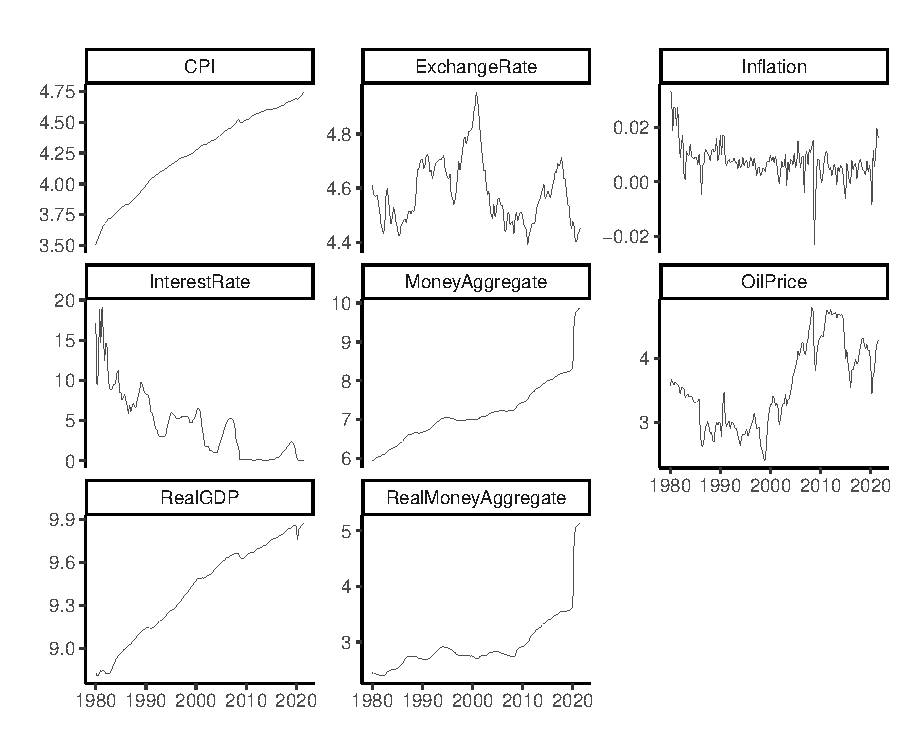
\includegraphics{Time_Series_Proj_Data_files/figure-latex/unnamed-chunk-1-1.pdf}
\caption{Time Series of the Macroeconomic Variables
(Log-Transformed).\label{fig1}}
\end{figure}

The results in table \ref{tab-2} suggests that interest rates (\(r_t\)),
real GDP (\(y_t\)), and oil price (\(o_t\)) are \(I(1)\), whereas the
monetary aggregate (\(m_t\)) and the price level (\(p_t\)) seems to be
\(I(2)\). This is identical to the suggestions by Cologni \& Manera
(\protect\hyperlink{ref-cologni2008}{2008}). To facilitate
comparability, the system is transformed from \(I(1)\) to \(I(2)\) as
done by Cologni \& Manera (\protect\hyperlink{ref-cologni2008}{2008}),
by reviewing the inflation rate \(\varDelta p_t\) and the real monetary
aggregate \((m_t-p_t)\). Failure to reject the null hypothesis of no
unit root for the differenced inflation rate
(\(\varDelta(\varDelta p_t)\)) and the differenced real monetary
aggregate \(\varDelta(m_t -p_t)\) suggests that these series are
\(I(1)\), confirming the robustness of these transformations implemented
by the authors.

\begin{table}
\caption{ADF~Tests for Unit Roots and Order of Integration.}
\begin{center}
\begin{tabular}{@{}lllllll@{}}
\toprule
\multicolumn{1}{l}{Variable}&
\multicolumn{1}{l}{Deterministic terms}&
\multicolumn{1}{l}{Lags}&
\multicolumn{1}{l}{Test value} &
\multicolumn{3}{c}{Critical values}
\\
\cmidrule(l){5-7}
& & & & 1\% & 5\% & 10\%\\
\midrule    
$\mathtt{r_t}$ & constant, trend & 2 & $-$-2.73 &
$-$4.04 & $-$3.45 & $-$3.15\\ 
$\varDelta \mathtt{r_t}$ & constant & 1 & $-$10.04 &
$-$3.51 & $-$2.89 & $-$2.58\\ 
$\mathtt{p_t}$ & constant, trend & 4 & $-$2.47 &
$-$4.04 & $-$3.45 & $-$3.15\\ 
$\varDelta \mathtt{p_t}$ & constant, trend & 2 & $-$2.5 &
$-$4.04 & $-$3.45 & $-$3.15\\ 
$\varDelta(\varDelta \mathtt{p_t})$ & constant & 1 & $-$2.61 &
$-$2.6 & $-$1.95 & $-$1.61\\  
$\mathtt{y_t}$ & constant, trend & 1 & $-$2.31 &
$-$3.51 & $-$2.89 & $-$2.58\\  
$\varDelta\mathtt{y_t}$ & constant & 0 & $-$2.8 &
$-$2.6 & $-$1.95 & $-$1.61\\ 
$ \mathtt{e_t}$ & constant, trend & 3 & $-$2.73 &
$-$4.04 & $-$3.45 & $-$3.15\\  
$\varDelta \mathtt{e_t}$ & constant & 1 & $-$5.5 &
$-$3.51 & $-$2.89 & $-$2.58\\ 
$\mathtt{o_t}$ & constant, trend & 1 & $-$2.65 &
$-$4.04 & $-$3.45 & $-$3.15\\ 
$\varDelta \mathtt{o_t}$ & constant & 0 & $-$8.15 &
$-$2.6 & $-$1.95 & $-$1.61\\ 
$\mathtt{m_t}$ & constant, trend & 2 & $-$1.83 &
$-$4.04 & $-$3.45 & $-$3.15\\ 
$\varDelta \mathtt{m_t}$ & constant & 1 & $-$2.33 &
$-$3.51 & $-$2.89 & $-$2.58\\ 
$(\mathtt{m_t-p_t})$ & constant, trend & 1 & $-$1.80 &
$-$3.51 & $-$2.89 & $-$2.58\\ 
$\varDelta (\mathtt{m_t - p_t)}$ & constant & 0 & $-$3.33 &
$-$2.6 & $-$1.95 & $-$1.61\\
\bottomrule
\end{tabular}
\end{center}
\label{tab-2}
\end{table}

\hypertarget{estimate-the-unrestricted-var-in-levels-and-check-the-adequacy-of-the-model-specification.}{%
\subsection{\texorpdfstring{Estimate the unrestricted VAR in levels and
check the adequacy of the model
specification.\label{step2}}{Estimate the unrestricted VAR in levels and check the adequacy of the model specification.}}\label{estimate-the-unrestricted-var-in-levels-and-check-the-adequacy-of-the-model-specification.}}

The order of lags of the unrestricted VAR(p) is selected based on the
Akaike Information Criteria (AIC) reported in table \ref{kable}. Similar
to Cologni \& Manera (\protect\hyperlink{ref-cologni2008}{2008}), a lag
order of two is selected. The unrestricted VAR(2) in levels is then
estimated and the adequacy of its specification is investigated. Special
attention is given to test that the errors are white noise. Since
Johansen \emph{et al.} (\protect\hyperlink{ref-johansen1992}{1992})'s
method is a maximum-likelihood approach, the limiting distributions are
derived assuming normal errors, however, specifications can be robust to
deviations that permit some non-normality and heteroscedasticity under
\(i.i.d.\) errors with finite variance. Critically, auto-correlated
residuals, time-varying parameters, and structural breaks are
unacceptable.

\begin{table}

\caption{\label{tab:unnamed-chunk-2}Unrestricted VAR(p) Optimal Lag Length Criteria \label{kable}}
\centering
\begin{tabu} to \linewidth {>{\raggedright}X>{\centering}X>{\centering}X>{\centering}X>{\centering}X}
\toprule
\multicolumn{1}{c}{ } & \multicolumn{4}{c}{Number of lags (p)} \\
\cmidrule(l{3pt}r{3pt}){2-5}
  & 1 & 2 & 3 & 4\\
\midrule
AIC(n) & -41.77 & -42.66 & -42.50 & -42.39\\
HQ(n) & -41.31 & -41.80 & -41.24 & -40.73\\
SC(n) & -40.62 & -40.52 & -39.37 & -38.28\\
\bottomrule
\multicolumn{5}{l}{\rule{0pt}{1em}\textit{Note: }}\\
\multicolumn{5}{l}{\rule{0pt}{1em}Assumed maximum lag length of four in correspondence with Cologni \& Manera (2008)}\\
\end{tabu}
\end{table}

Table \ref{tab-3} shows the multivariate and uni-variate tests for
normality (Jarque-Bera) and heteroskedasticity (ARCH). Despite evidence
of non-normality in the uni-variate series' of the oil price \(o_t\),
the interest rate \(r_t\), and the real monetary aggregate
\((m_t-p_t)\),the null hypothesis of non-normally distributed residuals
is rejected at the 5\% level of significance for the multivariate
VAR(2).

\begin{table}[t]
\caption{Tests for Normality and Homoskedasticity for the unrestricted VAR(2).}
\begin{center}
\begin{threeparttable}[b]
\begin{tabular}{@{}llllll@{}}
\toprule
\multicolumn{1}{l}{}&
\multicolumn{2}{c}{Jarque-Bera Test}&
\multicolumn{2}{c}{ARCH Test}
\\
\cmidrule(l){2-3}
\cmidrule(l){4-5}
\\
\multicolumn{2}{c}{}&
\multicolumn{2}{l}{$H_0:non-normal \ residuals$}&
\multicolumn{2}{l}{$H_0:Heteroskedasticity$}
\\ \\
\multicolumn{1}{l}{Variables}&
\multicolumn{1}{l}{$p$-value\tnote{1}}&
\multicolumn{1}{l}{Interpretation}&
\multicolumn{1}{l}{$p$-value}&
\multicolumn{1}{l}{Interpretation}&
\\   
\midrule    
$Multivariate$ & 0.51 & Reject null of non-normality & 
0.42 & Fail to reject null\\
$y_t$ & 0.67 & Reject null of non-normality & 
 0.603 & Reject null\\
$o_t$ & 0.023 & Fail to reject null & 
 0.982& Reject null\\
$r_t$ & 0.00 & Fail to reject null & 
 0.193 & Fail to reject null\\
$\varDelta{p}_t$ & 0.804 & Reject null of non-normality & 
 0.43 & Fail to reject null\\
$e_t$ & 0.77 & Reject null of non-normality & 
 0.678 & Reject null\\
$(m_t-p_t)$ & 0.43 & Fail to reject null & 
 0.29 & Fail to reject null\\
\bottomrule
\end{tabular}
\begin{tablenotes}
    \item[1] Hypothesis are tested at the 5 percent significance level
  \end{tablenotes}
\end{threeparttable}
\label{tab-3}
\end{center}
\end{table}

The null hypothesis of heteroscedasticity (ARCH test) cannot be rejected
at the 5\% level of significance for the multivariate VAR(2), where the
oil price \(o_t\), the interest rate \(r_t\), and the real monetary
aggregate \((m_t-p_t)\) are each individually a source of this
heteroscedasticity. The question becomes whether this level of
heteroscedasticity still permits robust maximum-likelihood estimations.
To answer this, more specification tests are conducted.

Both the Portmanteau (Asymptotic) and the Breusch-Godfrey LM tests
reported in table \ref{tab-4} provide strong evidence that the residuals
are not serially correlated. In addition, the (OLS) CUSUM tests and the
empirical fluctuations plot for each series are given in figures
\ref{figA7} and \ref{figA8} in Appendix \ref{A}, providing significant
evidence that the series have no structural breaks nor time-varying
parameters.

Provided the strict requirements of no-serial-correlation,
no-structural-breaks, and no-time-varying parameters are satisfied; the
degree of homoscedasticity present within the unrestricted VAR(2) is
assumed as acceptable.

\begin{table}[t]
\caption{Tests for serial correlation unrestricted VAR(2)'s resduals.}
\begin{center}
\begin{threeparttable}[b]
\begin{tabular}{@{}llllll@{}}
\toprule
\multicolumn{2}{c}{Portmanteau Test (Asymptotic)}&
\multicolumn{2}{c}{Breusch-Godfrey LM Test}
\\
\cmidrule(l){1-2}
\cmidrule(l){3-4}
\\
\multicolumn{2}{l}{$H_0:no \ serial\ correlation$}&
\multicolumn{2}{l}{$H_0:no \ serial\ correlation \ up \ to \ order \ p$}&
\\ \\
\multicolumn{1}{l}{$p$-value\tnote{1}}&
\multicolumn{1}{l}{Interpretation}&
\multicolumn{1}{l}{$p$-value}&
\multicolumn{1}{l}{Interpretation}&
\\   
\midrule    
0.6539 & Fail to reject the null  & 
0.6317 & Fail to reject the null \\
\bottomrule
\end{tabular}
\begin{tablenotes}
    \item[1] Hypothesis are tested at the 5 percent significance level
  \end{tablenotes}
  \end{threeparttable}
\label{tab-4}
\end{center}
\end{table}

\hypertarget{select-the-specification-of-the-deterministic-component-determine-the-number-of-cointegrating-relationships-r-and-determine-the-specification-of-the-long-run-and-short-run-relationships-as-necessary-for-identification.}{%
\subsection{\texorpdfstring{Select the specification of the
deterministic component, determine the number of cointegrating
relationships \(r\), and determine the specification of the long-run and
short-run relationships as necessary for identification.
\label{step3}}{Select the specification of the deterministic component, determine the number of cointegrating relationships r, and determine the specification of the long-run and short-run relationships as necessary for identification. }}\label{select-the-specification-of-the-deterministic-component-determine-the-number-of-cointegrating-relationships-r-and-determine-the-specification-of-the-long-run-and-short-run-relationships-as-necessary-for-identification.}}

In accordance with Cologni \& Manera
(\protect\hyperlink{ref-cologni2008}{2008}), the deterministic terms
contained within
\(\bm{\Phi}_t \bm{D}_t= \bm{\mu}_t = \bm{\mu}_0 + \bm{\mu}_1 t\) (see
\ref{2}) are assumed to contain a restricted trend to limit the trending
nature of most of the series. The restricted VECM becomes: \begin{align}
\Delta \bm{Y}_t = \bm{\mu}_0 + \bm{\alpha}(\bm{\beta}'\bm{Y}_{t-1} + \bm{\rho}_1 t) +  \bm{\Gamma}_1 \bm{\Delta Y}_{t-1} + ... + \bm{\Gamma}_{p-1} \bm{\Delta} \bm{Y}_{t-p+1} + \bm{u}_t, \ \ \ t=1,...,T, \label{10}
\end{align} where the series in \(\bm{Y_t}\) are \(I(1)\) with drift
vector \(\bm{\mu}_0\) and the cointegrating relations
\(\bm{\beta' Y_t}\) contain a linear trend term \(\bm{\rho_1} t\).

The number of cointegrating relationships (\(r\)) contained within the
\(\bm{\beta}\) matrix is determined using Johansen
(\protect\hyperlink{ref-johansen1995}{1995})'s LR approach. The Trace
and Maximum-Eigenvalue test statistics are outlined in table \ref{tab-5}
below. Similar to hypothesized results by Cologni \& Manera
(\protect\hyperlink{ref-cologni2008}{2008}), both tests provide evidence
of one co-integrating relationship at the 1\% level of significance.\\

\begin{table}[t]
\caption{Testing for the number of co-integrating relationships contained in $\bm{\beta'}$.}
\begin{center}
\begin{threeparttable}[b]
\begin{tabular}{@{}llclll@{}}
\toprule
\multicolumn{1}{l}{}&
\multicolumn{1}{l}{}&
\multicolumn{1}{l}{Trace Statistics\tnote{1}}&
\multicolumn{1}{l}{0.05 Critical Value}&
\\   
\midrule    
$H_o$ & $H_1$ & $Trace \ test$ \\
\\
$r=0$ & $r=1$ & 144.21$^{**}$ & 114.90\\
$r \le 1$ & $r=2$ & 85.74 & 87.31\\
$r \le 2$ & $r=3$ & 42.24 & 62.99\\
$r \le 3$ & $r=4$ & 20.70 & 42.44\\
$r \le 4$ & $r=5$ & 10.56 & 25.32\\
\\
$H_o$ & $H_1$ & $Max-eigenvalue \ test$\\
\\
$r=0$ & $r=1$  & 58.48$^{*}$ & 43.97\\
$r \le 1$ & $r=2$ & 43.50$^{***}$ & 37.52\\
$r \le 2$ & $r=3$ & 21.53 & 31.46\\
$r \le 3$ & $r=4$ & 10.15 & 25.54\\
$r \le 4$ & $r=5$ & 7.25 & 18.96\\
\bottomrule
\end{tabular}
\begin{tablenotes}
    \item[1] *,**,** represents rejection of the null hypothesis at the 1, 5, and 10 percent levels. The specification includes a constant and a trend.
  \end{tablenotes}
\end{threeparttable}
\label{tab-5}
\end{center}
\end{table}

\hypertarget{specification-and-identification-of-the-long-run-relationship}{%
\subsubsection{\texorpdfstring{Specification and identification of the
long-run relationship
\label{lrr}}{Specification and identification of the long-run relationship }}\label{specification-and-identification-of-the-long-run-relationship}}

The next step is to estimate the co-integrating relationship (\(r=1\))
of the restricted model. Cologni \& Manera
(\protect\hyperlink{ref-cologni2008}{2008}) considers two long-run
relationships as possible specifications for the co-integrating
relationships. A standard money demand equation is the first long-run
relationship considered: \begin{align}
m_t - p_t = \beta_o + \beta_1 y_t - \beta_2 r_t - \beta_3 \Delta p_t. \label{CR1}
\end{align} The second second long-run relationship equates excess
output to the exchange rate, the inflation rate, the interest rate, and
oil prices: \begin{align}
y_t - \beta_4 trend = \beta_5 + \beta_6 e_t - \beta_7 r_t - \beta_8 \Delta p_t - \beta_9 o_t. \label{CR2}
\end{align} Table \ref{tab-6} presents both the estimates of this paper
and that of the authors. The authors found that the coefficient relating
to the money demand specification is not statistically different from
zero, and the LR test resulted in the rejection of null hypothesis of
the conventional money demand function (\ref{CR1}). Rather, the excess
output function (\ref{CR2}) is interpreted as the long run relationship
for the United States.

\begin{table}[t]
\caption{Estimated co-integrated relationships of the restricted system.}
\begin{center}
\begin{threeparttable}[b]
\begin{tabular}{@{}llllllllllllllllllll@{}}
\toprule
\multicolumn{9}{c}{My Estimates \tnote{1}}&
\\
\cmidrule(l){1-9}
\multicolumn{1}{l}{$y_t$}&
\multicolumn{1}{l}{$o_t$}&
\multicolumn{1}{l}{$r_t$}&
\multicolumn{1}{l}{$\varDelta p_t$}&
\multicolumn{1}{l}{$e_t$}&
\multicolumn{1}{l}{$m_t$}&
\multicolumn{1}{l}{$constant$}&
\multicolumn{1}{l}{$trend$}&
\multicolumn{1}{l}{$LR \ test$}&
\\
\midrule    
    1 & 0.082 & -1.693 & -34.237  & - & - & -4.070 &-0.025 & $\chi^2(2)=$\\ 
      &    (0.022)   & (0.542)  &    (3.750)      &      &  & & (0.0009)       & 1.69[0.43]          \\
\midrule
\multicolumn{9}{c}{Estimations by Cologni $\&$ Manera (2008)}&
\\
\cmidrule(l){1-9}
\multicolumn{1}{l}{$y_t$}&
\multicolumn{1}{l}{$o_t$}&
\multicolumn{1}{l}{$r_t$}&
\multicolumn{1}{l}{$\varDelta p_t$}&
\multicolumn{1}{l}{$e_t$}&
\multicolumn{1}{l}{$m_t$}&
\multicolumn{1}{l}{$constant$}&
\multicolumn{1}{l}{$trend$}&
\multicolumn{1}{l}{$LR \ test$}&
\\   
\midrule    
      1 & 0.160 & - & -26.019  & 0.218 & - & -8.511 &-0.009 & $\chi^2(2)=$\\ 
      &    (0.036)   &   &    (3.191)      & (0.059)      &  & & (0.0004)       & 2.44[0.36]          \\
\bottomrule
\end{tabular}
\begin{tablenotes}
    \item[1] Values in round brackets represents the parameter estimates standard errors, and in square brackets the p-values from the log-likelihood test for over-identifications.  
  \end{tablenotes}
\end{threeparttable}
\label{tab-6}
\end{center}
\end{table}

Similarly, the LR test in this paper also rejects the null hypothesis of
a conventional money demand function and adopts the excess output
function as the specification for the long-run relationship. In
particular, the data does not reject the existence of a negative
long-run effect of oil prices on excess output. However, in contrast to
Cologni \& Manera (\protect\hyperlink{ref-cologni2008}{2008}), the LR
test for over-identification indicates that interest rates (\(r_t\)) has
a significant negative effect on excess output, whereas exchange rates
(\(e_t\)) has no effect. This minor difference in the identification of
the long-run relationship produces an larger \(p\)-value {[}0.43{]} than
estimated by the authors {[}0.33{]}, resulting in a significantly
lower-likelihood of rejecting the null of valid over-identifying
restrictions.

\hypertarget{specification-and-identification-of-the-short-run-relationships}{%
\subsubsection{\texorpdfstring{Specification and identification of the
short-run relationships
\label{srr}}{Specification and identification of the short-run relationships }}\label{specification-and-identification-of-the-short-run-relationships}}

The model's short-run dynamics is described by adopting the
identification strategy applied by Cologni \& Manera
(\protect\hyperlink{ref-cologni2008}{2008}), that imposes a set of
over-identifying restrictions on the coefficients of the \(\bm{B}\)
matrix in equation (\ref{2}). The assumed short-run relationships are
specified as: \begin{align}
u_m = b_{11} \varepsilon_m + b_{12} \varepsilon_r + b_{14} \varepsilon_{\Delta p}. \label{a} \\ 
u_r= b_{22} \varepsilon_r+ b_{23} \varepsilon_y + b_{24}\varepsilon_{\Delta p} + b_{25 }\varepsilon_e  + b_{26} \varepsilon_o. \label{b} \\ 
u_y= b_{33} \varepsilon_y  + b_{34} \varepsilon_{\Delta p} +  b_{35} \varepsilon_e + b_{36}\varepsilon_o. \label{c} \\
u_{\Delta p}= b_{44} \varepsilon_{\Delta p} + b_{45}\varepsilon_e + b_{46} \varepsilon_o. \label{d} \\ 
u_e=b_{55} \varepsilon_e + b_{56 }\varepsilon_o. \label{e} \\ 
u_o=  b_{66}\varepsilon_o, \label{f}
\end{align} where \(u_m\), \(u_r\), \(u_y\), \(u_{\Delta p}\), \(u_e\),
and \(u_o\) represents the reduced-form errors, whereas
\(\varepsilon_m\), \(\varepsilon_r\), \(\varepsilon_y\),
\(\varepsilon_{\Delta p}\), \(\varepsilon_e\), and \(\varepsilon_o\) the
structural shocks in money demand, money supply, real output, price
setting, exchange rates, and oil prices.\footnote{The economic theory
  applied to derive these short-run dynamics are omitted due to this
  paper's focus on the robustness of the econometric method. See Cologni
  \& Manera (\protect\hyperlink{ref-cologni2008}{2008}) for a detailed
  description.}

Specifications (\ref{a}), (\ref{b}), and (\ref{c}) implies
\(b_{13}=b_{15}=b_{16}=0\), \(b_{21}=0\), and \(b_{31}=b_{32}=0\),
respectively. Where specifications (\ref{d}), (\ref{e}), and (\ref{f})
equates to \(b_{41}=b_{42}=b_{43}=0\),\(b_{51}=b_{52}=b_{53}=b_{54}=0\),
and \(b_{61}=b_{62}=b_{63}=b_{64}=b_{65}=0\), respectively.

\hypertarget{estimate-the-resulting-reduced-rank-cointegrated-vecm-interpret-the-economic-dynamics-of-the-model-and-test-further-hypothesized-restrictions.}{%
\subsection{\texorpdfstring{Estimate the resulting (reduced-rank)
cointegrated VECM, interpret the economic dynamics of the model, and
test further hypothesized restrictions.
\label{step4}}{Estimate the resulting (reduced-rank) cointegrated VECM, interpret the economic dynamics of the model, and test further hypothesized restrictions. }}\label{estimate-the-resulting-reduced-rank-cointegrated-vecm-interpret-the-economic-dynamics-of-the-model-and-test-further-hypothesized-restrictions.}}

The set of short-run over-identification restrictions given by equations
(\ref{a})-(\ref{f}) are tested using the conventional likelihood-ratio
(LR) statistic, after which the structural shocks are recovered by
estimating the contemporaneous impact matrix \(\bm{B}\). Lastly, impulse
response analysis is conducted. The results are continuously compared
with the findings by Cologni \& Manera
(\protect\hyperlink{ref-cologni2008}{2008}).

The estimated coefficients for contemporaneous impact matrix B in the
structural model with its corresponding LR statistic is given in table
\ref{7}. The LR test statistic for the over-identifying short-run
restrictions fails to reject the null hypothesis of valid restrictions
at the 5\% significance level.

\begin{table}
\caption{Estimated coefficients for contemporaneous impact matrix $\bm{B}$ in the structural model.\tnote{1}}
\begin{center}
\begin{threeparttable}[b]
\begin{tabular}{@{}llllllll@{}}
\toprule
\multicolumn{1}{l}{}&
\multicolumn{1}{l}{$b_{i,1}$}&
\multicolumn{1}{l}{$b_{i,2}$}&
\multicolumn{1}{l}{$b_{i,3}$}&
\multicolumn{1}{l}{$b_{i,4}$}&
\multicolumn{1}{l}{$b_{i,5}$}&
\multicolumn{1}{l}{$b_{i,6}$}
\\
\midrule    
$b_{1,j}$ & 0.008$^{*}$ & -0.002$^{***}$ & - &
-0.0022$^{***}$ & - & - \\ 
& (0.001) & (0.0008) &  & (0.001) & & \\
$b_{2,j}$ & - & 0.957$^{*}$ & 0.2375 &
0.3128$^{**}$ & 0.0161 & 0.0352$^{**}$ \\ 
& & (0.123) &  (0.952) & (0.1141) & (0.1002) & (0.102)\\
$b_{3,j}$ & - & - & 0.0048$^{*}$ &
0.001 & 0.0002$^{*}$ & -0.0001\\  
& & & (0.0006) & (0.0006) & (0.0004) & (0.0005) \\
$b_{4,j}$ & - & - & - &
 0.0026$^{*}$ & -0.0004 & 0.0014$^{*}$ \\  
& & & & (0.0003) & (0.0002) & (0.0003)\\
$b_{5,j}$ & - & - & - &
- & 0.029$^{*}$ & 0.0043 \\  
& & & & & (0.0034) & (0.0028)\\
$b_{6,j}$ & - & - & - &
- & - & 0.126$^{*}$ \\  
& & & & & & (0.0176)\\
\midrule
\multicolumn{7}{c}{LR Test for overidentification: $\chi^2(3)=3.27[0.19]$}&
\\
\bottomrule
\end{tabular}
\begin{tablenotes}
    \item[1] b(i,j), i,j=1,..,6 are the estimated matrix B's parameters. Values in round brackets represents the parameter estimates standard errors, and in square brackets the p-values from the log-likelihood test for over-identifications.*,**,***, represents the 1,5, and 10 percent significance level of the coefficient.  
  \end{tablenotes}
\end{threeparttable}
\end{center}
\label{tab-7}
\end{table}

The analysis of table \ref{7} has similar results as Cologni \& Manera
(\protect\hyperlink{ref-cologni2008}{2008}) in the following aspects:
The short-run impact coefficient reflecting the effect of oil prices on
the inflation rate (\(b_{4,6}\)) is positive and statistically
significant at the 1\% level. Also, there is no robust evidence that oil
prices exerts an instantaneous effect on real GDP growth (\(b_{3,6}\)).
Lastly, that a oil price shock has no contemporaneous impact on the
exchange rates (\(b_{5,6}\)).

The empirical results differ from Cologni \& Manera
(\protect\hyperlink{ref-cologni2008}{2008}) in the following ways: the
estimates suggest that following a shock to the inflation rate, interest
rates increase, being indicative of monetary tightening (\(b_{2,4}\)).
Additionally, our estimations highlight the short-run negative trade-off
between the inflation rate and GDP growth (\(b_{3,4}\)).

The estimated impulse responses following a one standard deviation shock
to the oil price is depicted in figure \ref{irf1}, with the
corresponding 95\% confidence interval bandwidth provided.\footnote{As
  executed by Cologni \& Manera
  (\protect\hyperlink{ref-cologni2008}{2008}), the impulse response
  functions are computed by assuming 4 lags. The results are similar for
  the U.S. for lag lengths of 2,3, and 4.} Similar to Cologni \& Manera
(\protect\hyperlink{ref-cologni2008}{2008}), an increase in the oil
price tends to be followed by a rise in inflation. However, the impact
is short lived, and progressively fades away towards its natural level.
Moreover, the impulse responses are indicative that output is negatively
affected by the sudden increase in oil prices, where Cologni \& Manera
(\protect\hyperlink{ref-cologni2008}{2008}) explains that this is due to
the U.S. being heavily dependent on foreign supplies of oil. However, in
contrast to the authors findings, here the effects on output seems to be
permanent and not temporary, being indicative of alternative
specifications of the long-run relationships within the system.

Another apparent distinction in the impulse responses is that
innovations to the oil price does not exert an as large negative effect
on exchange rates for the U.S. than the results by Cologni \& Manera
(\protect\hyperlink{ref-cologni2008}{2008}) suggests.

\begin{figure}[H]

{\centering \subfloat[(a)\label{fig:unnamed-chunk-4-1}]{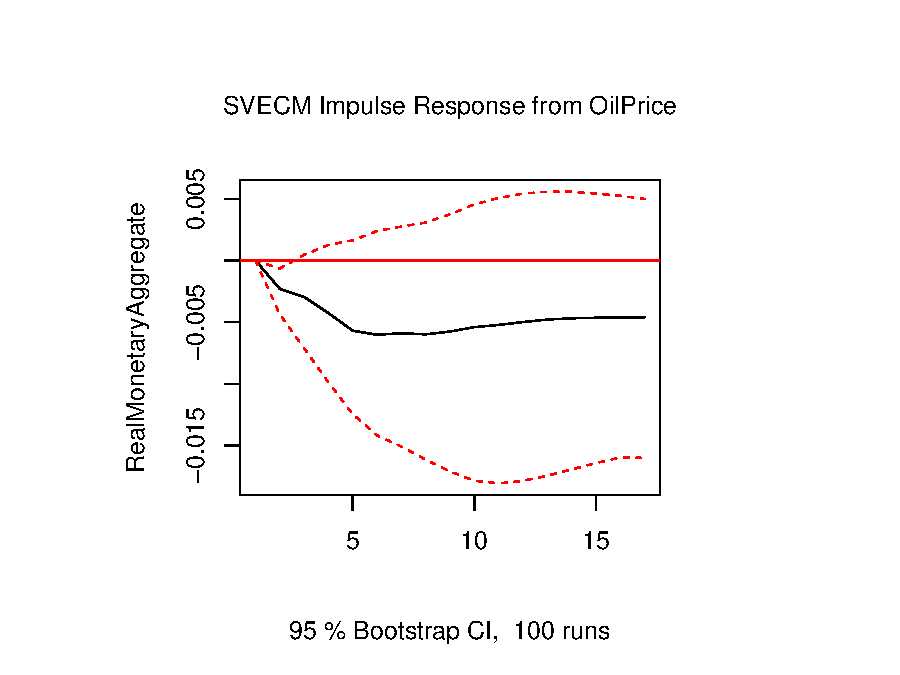
\includegraphics[width=0.5\linewidth]{Time_Series_Proj_Data_files/figure-latex/unnamed-chunk-4-1} }\subfloat[(b)\label{fig:unnamed-chunk-4-2}]{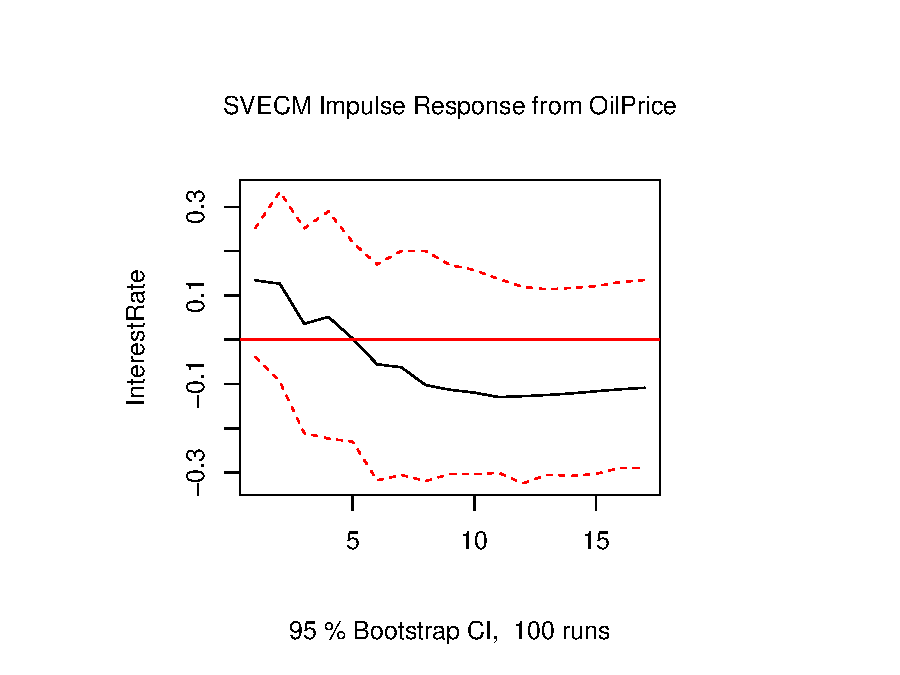
\includegraphics[width=0.5\linewidth]{Time_Series_Proj_Data_files/figure-latex/unnamed-chunk-4-2} }\newline\subfloat[(c)\label{fig:unnamed-chunk-4-3}]{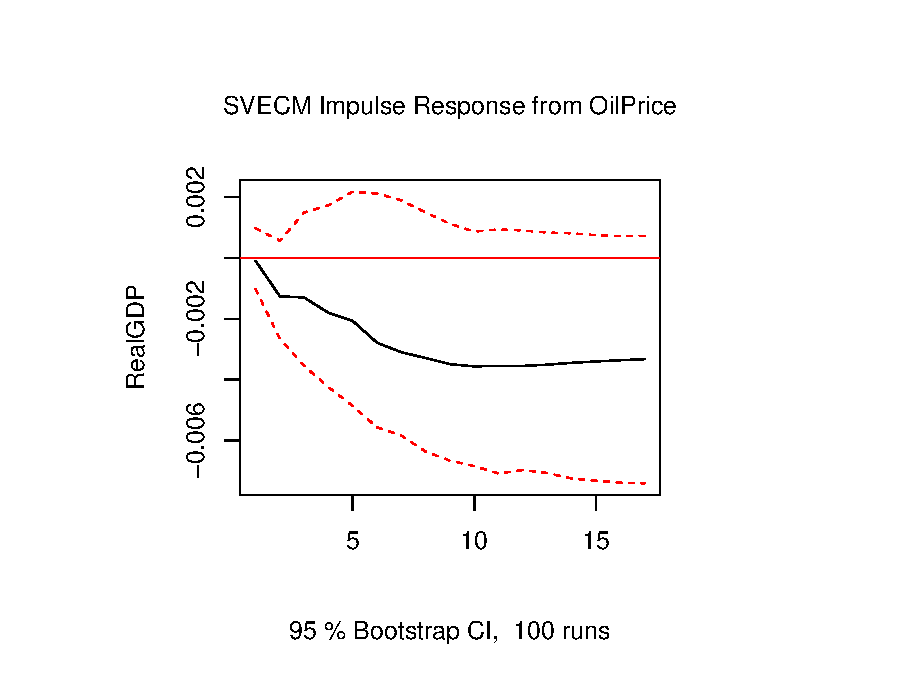
\includegraphics[width=0.5\linewidth]{Time_Series_Proj_Data_files/figure-latex/unnamed-chunk-4-3} }\subfloat[(d)\label{fig:unnamed-chunk-4-4}]{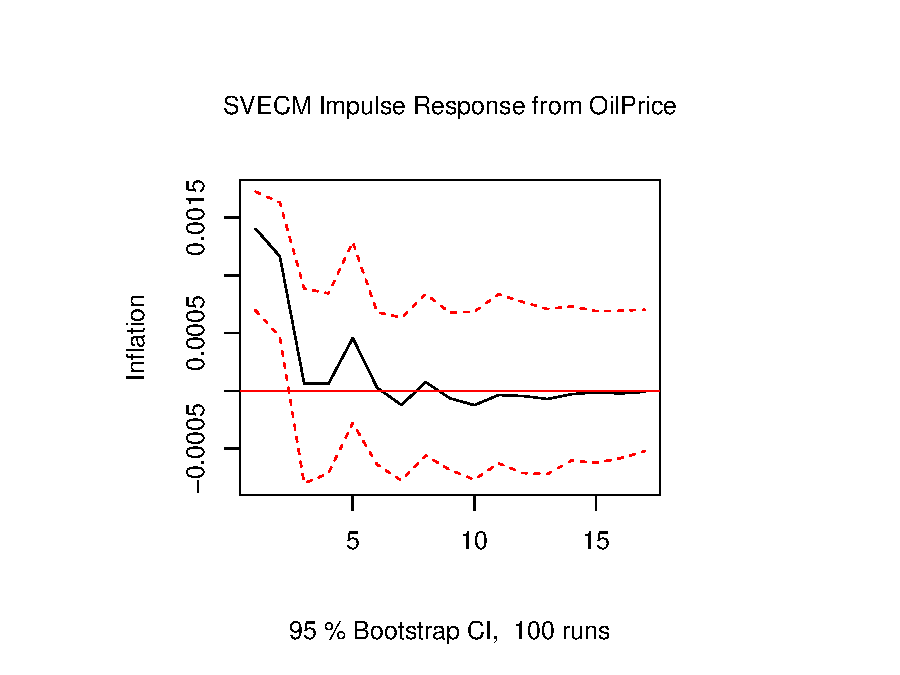
\includegraphics[width=0.5\linewidth]{Time_Series_Proj_Data_files/figure-latex/unnamed-chunk-4-4} }\newline\subfloat[(e)\label{fig:unnamed-chunk-4-5}]{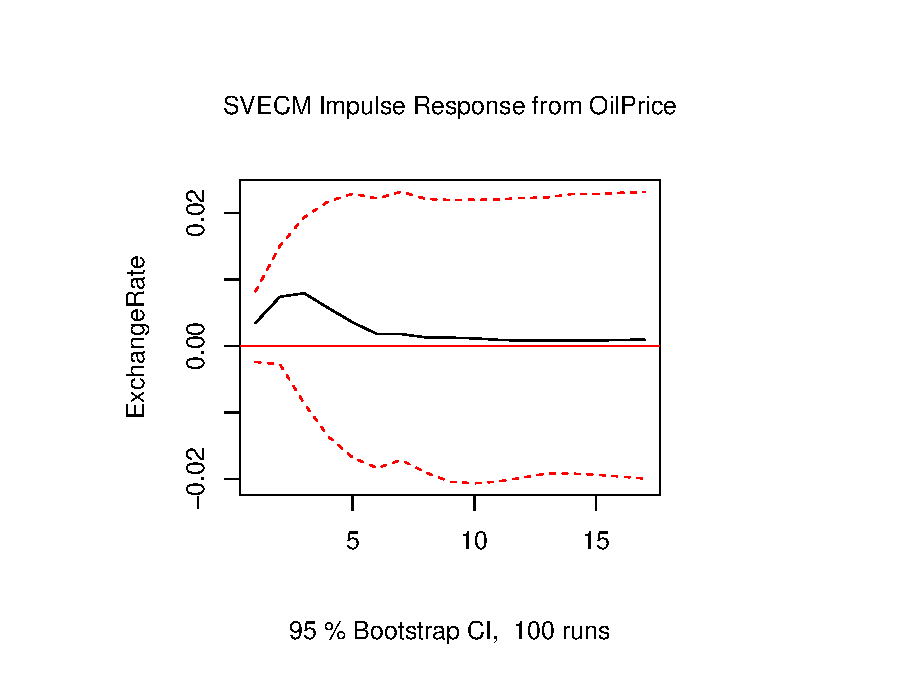
\includegraphics[width=0.5\linewidth]{Time_Series_Proj_Data_files/figure-latex/unnamed-chunk-4-5} }

}

\caption{Impulse responses from an oil price shock \label{irf1}}\label{fig:unnamed-chunk-4}
\end{figure}

\newpage

\hypertarget{references}{%
\section*{References}\label{references}}
\addcontentsline{toc}{section}{References}

\hypertarget{refs}{}
\begin{CSLReferences}{1}{0}
\leavevmode\vadjust pre{\hypertarget{ref-cologni2008}{}}%
Cologni, A. \& Manera, M. 2008. Oil prices, inflation and interest rates
in a structural cointegrated VAR model for the g-7 countries.
\emph{Energy economics}. 30(3):856--888.

\leavevmode\vadjust pre{\hypertarget{ref-johansen1992}{}}%
Johansen, S. et al. 1992. Determination of cointegration rank in the
presence of a linear trend. \emph{Oxford bulletin of economics and
statistics}. 54(3):383--397.

\leavevmode\vadjust pre{\hypertarget{ref-johansen1995}{}}%
Johansen, S. 1995. \emph{Likelihood-based inference in cointegrated
vector autoregressive models}. OUP Oxford.

\leavevmode\vadjust pre{\hypertarget{ref-lutkepohl2005}{}}%
Lütkepohl, H. 2005. \emph{New introduction to multiple time series
analysis}. Springer Science \& Business Media.

\leavevmode\vadjust pre{\hypertarget{ref-sims1993}{}}%
Sims, C.A. 1993. A nine-variable probabilistic macroeconomic forecasting
model. In University of Chicago press \emph{Business cycles, indicators,
and forecasting}. 179--212.

\end{CSLReferences}

\newpage

\hypertarget{appendix}{%
\section*{Appendix}\label{appendix}}
\addcontentsline{toc}{section}{Appendix}

\appendix
\renewcommand{\thesection}{A}

\hypertarget{appendix-a--}{%
\subsection{\texorpdfstring{Appendix A \{-\}
\label{A}}{Appendix A \{-\} }}\label{appendix-a--}}

\begin{figure}
\centering
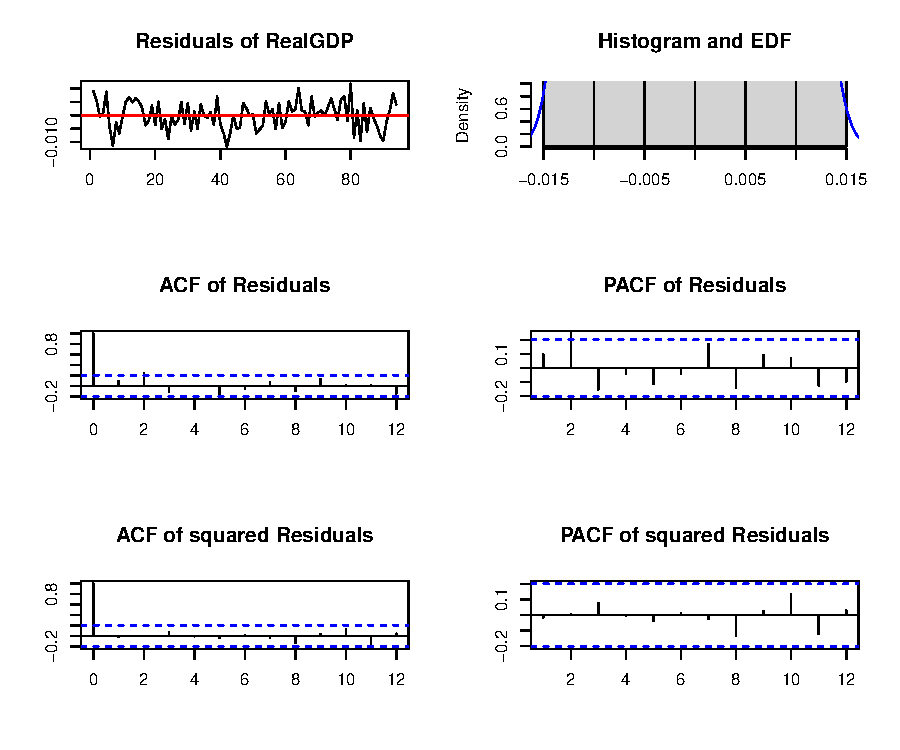
\includegraphics{Time_Series_Proj_Data_files/figure-latex/unnamed-chunk-5-1.pdf}
\caption{Diagnostics plot of VAR(2) for Real GDP\label{figA1}}
\end{figure}

\begin{figure}
\centering
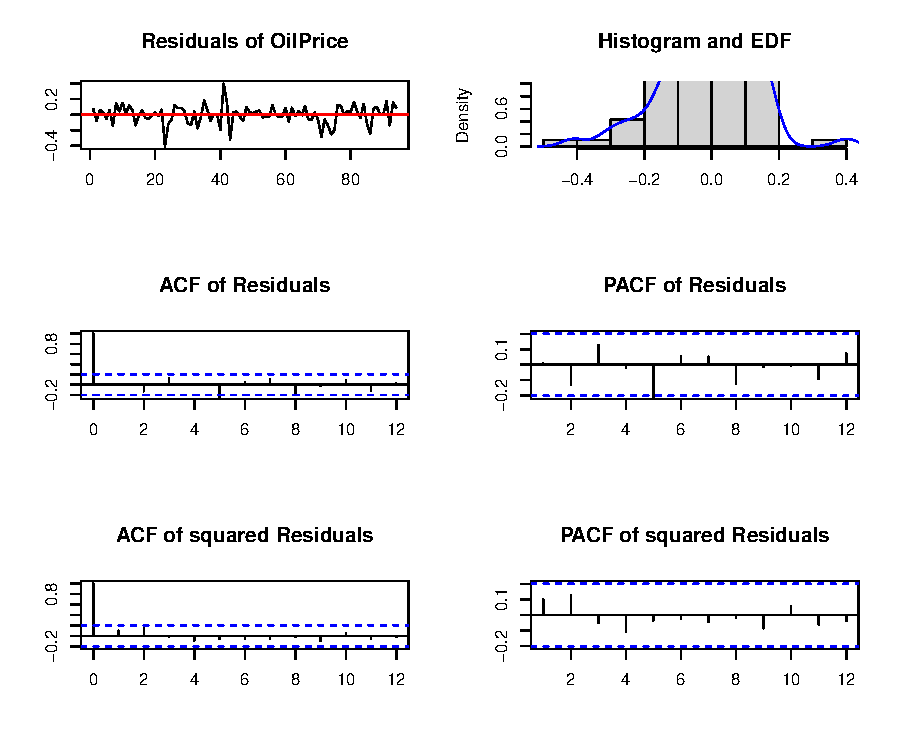
\includegraphics{Time_Series_Proj_Data_files/figure-latex/unnamed-chunk-6-1.pdf}
\caption{Diagnostics plot of VAR(2) for Oil Price\label{figA2}}
\end{figure}

\begin{figure}
\centering
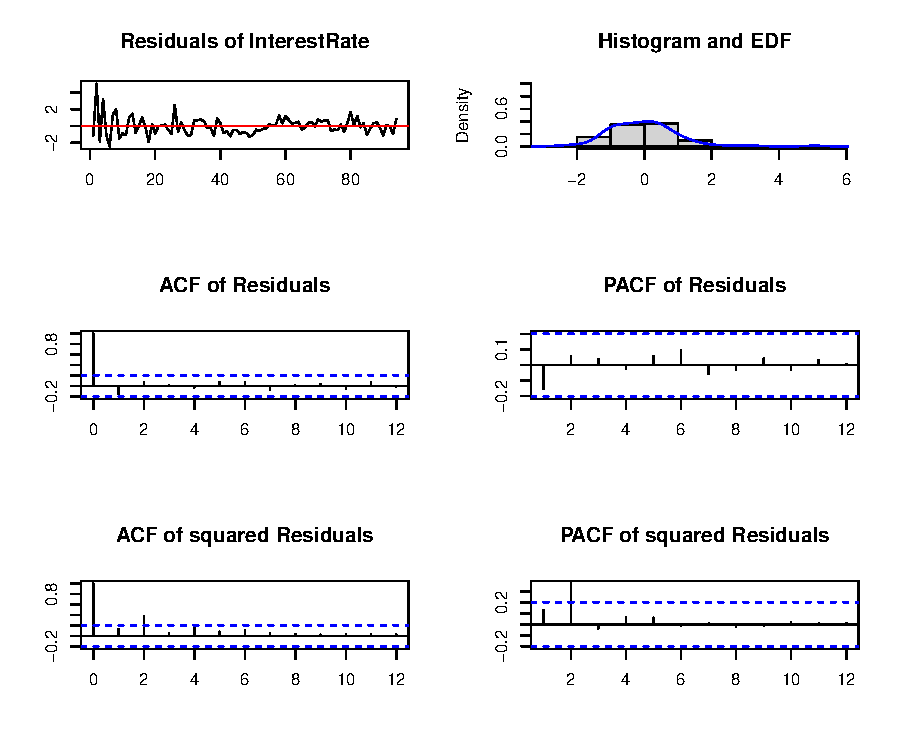
\includegraphics{Time_Series_Proj_Data_files/figure-latex/unnamed-chunk-7-1.pdf}
\caption{Diagnostics plot of VAR(2) for Interest Rate\label{figA3}}
\end{figure}

\begin{figure}
\centering
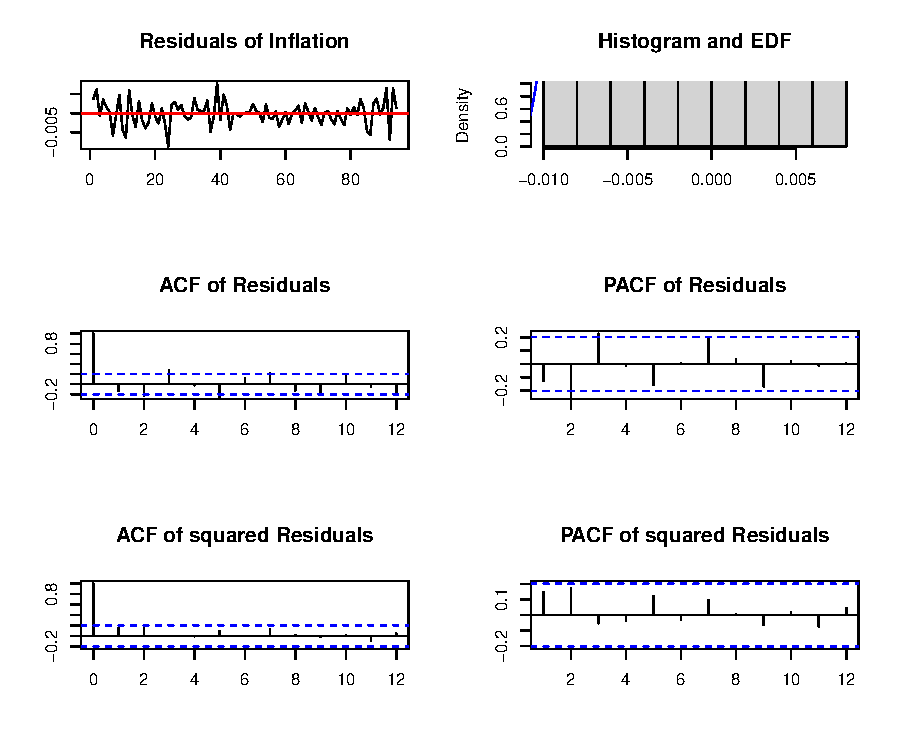
\includegraphics{Time_Series_Proj_Data_files/figure-latex/unnamed-chunk-8-1.pdf}
\caption{Diagnostics plot of VAR(2) for Inflation\label{figA4}}
\end{figure}

\begin{figure}
\centering
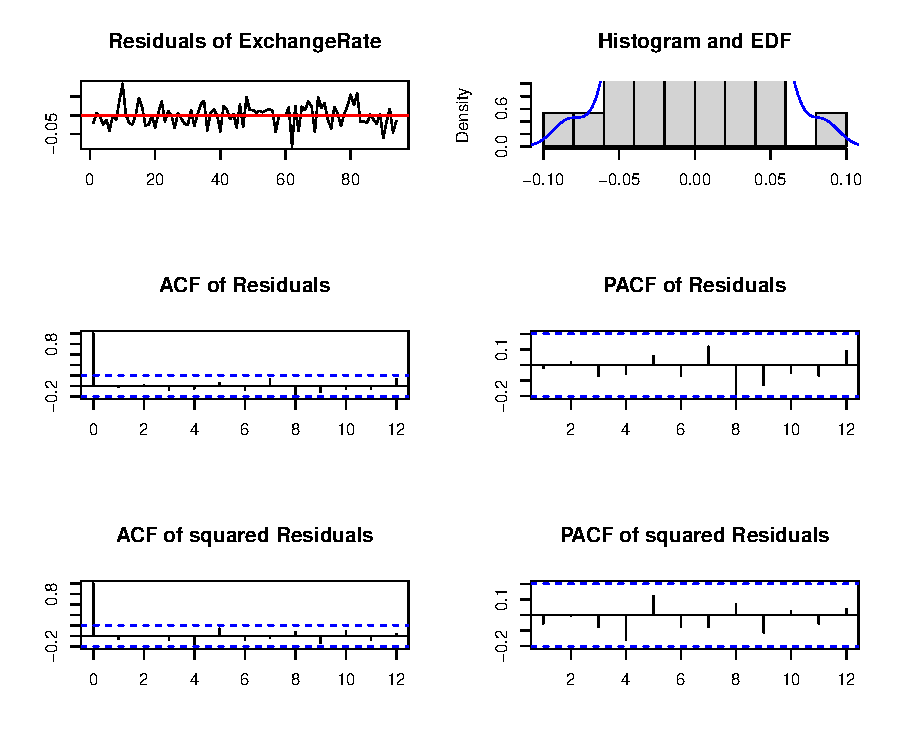
\includegraphics{Time_Series_Proj_Data_files/figure-latex/unnamed-chunk-9-1.pdf}
\caption{Diagnostics plot of VAR(2) for Exchange Rate\label{figA5}}
\end{figure}

\begin{figure}
\centering
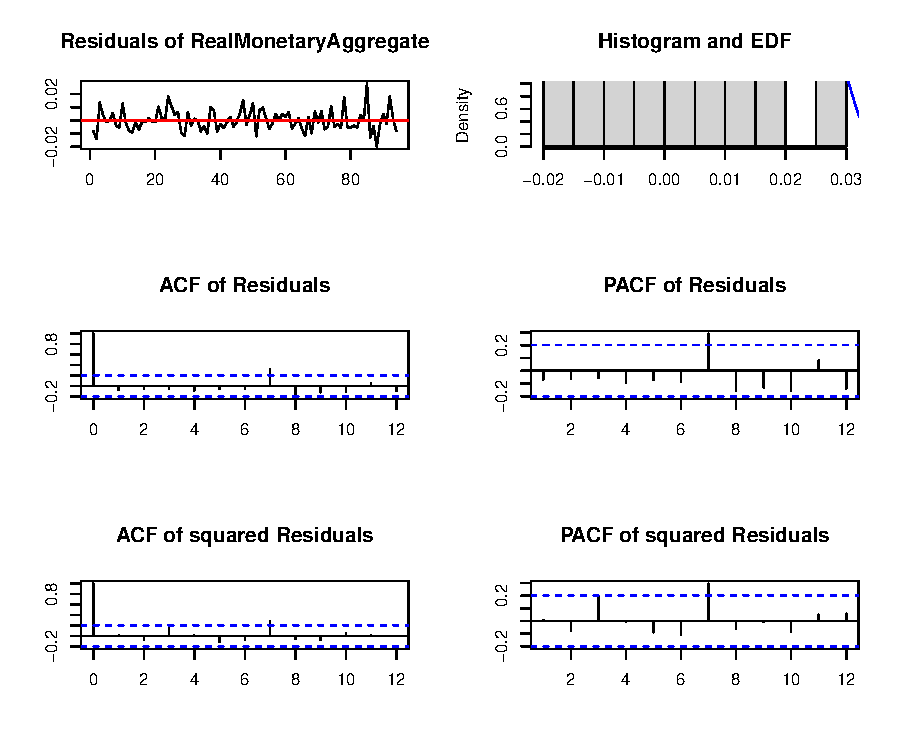
\includegraphics{Time_Series_Proj_Data_files/figure-latex/unnamed-chunk-10-1.pdf}
\caption{Diagnostics plot of VAR(2) for Real Money\label{figA6}}
\end{figure}

\begin{figure}
\centering
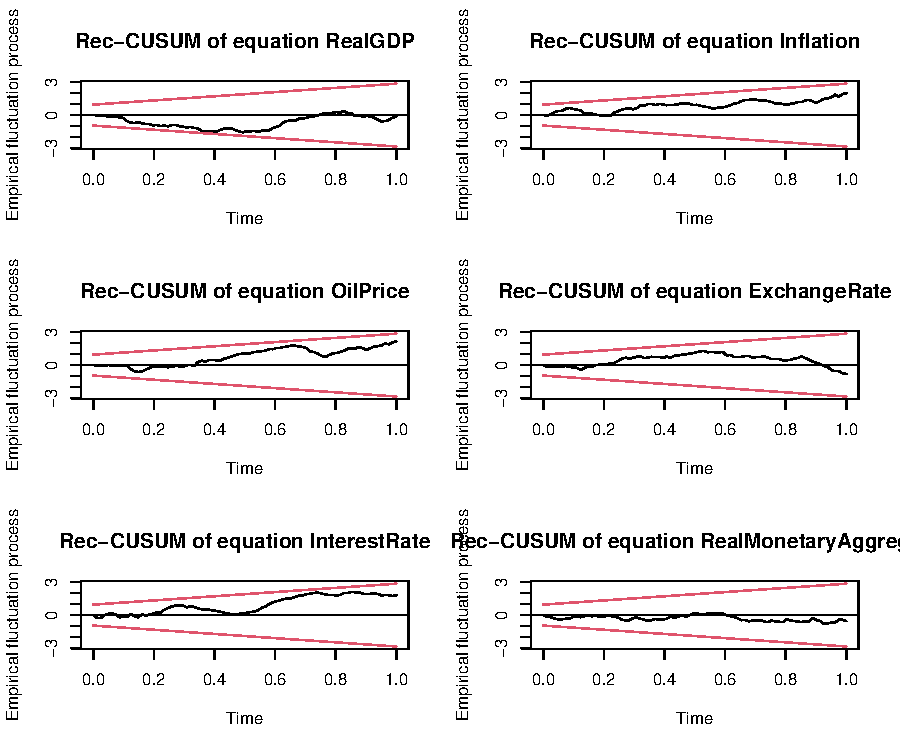
\includegraphics{Time_Series_Proj_Data_files/figure-latex/unnamed-chunk-11-1.pdf}
\caption{OLS-CUSUM test for VAR(2)\label{figA7}}
\end{figure}

\begin{figure}
\centering
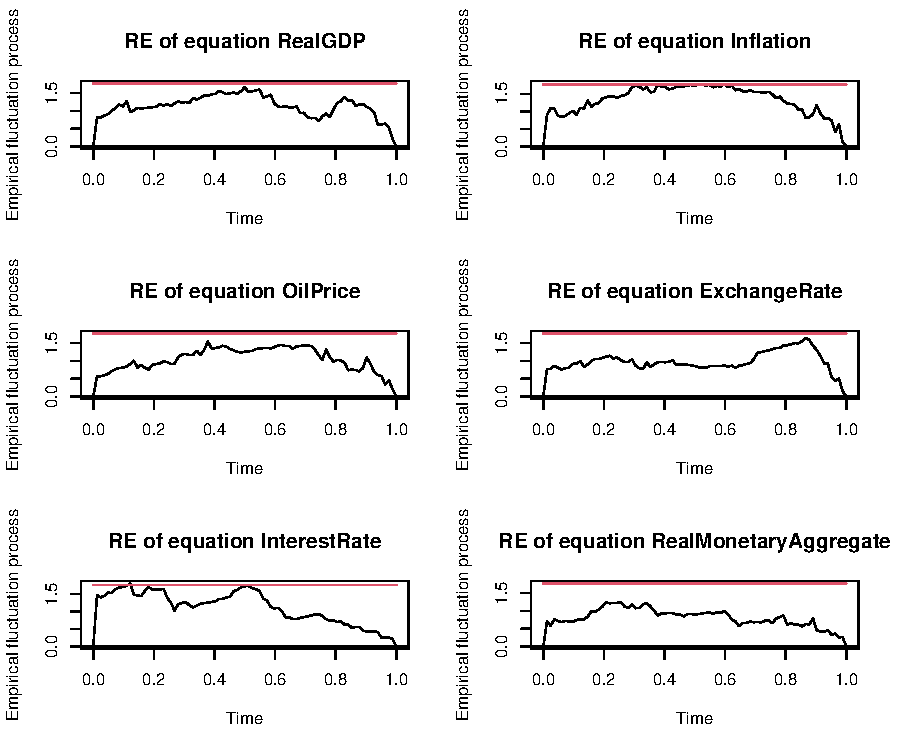
\includegraphics{Time_Series_Proj_Data_files/figure-latex/unnamed-chunk-12-1.pdf}
\caption{Empirical fluctuation plot for VAR(2) \label{figA8}}
\end{figure}

\bibliography{Tex/ref}





\end{document}
